%%%%%%%%%%%%%%%%%%%%%%%%%%%%%%%%%%%%%%%%%
%
% CMPT 435
% Lab Zero
%
%%%%%%%%%%%%%%%%%%%%%%%%%%%%%%%%%%%%%%%%%

%%%%%%%%%%%%%%%%%%%%%%%%%%%%%%%%%%%%%%%%%
% Short Sectioned Assignment
% LaTeX Template
% Version 1.0 (5/5/12)
%
% This template has been downloaded from: http://www.LaTeXTemplates.com
% Original author: % Frits Wenneker (http://www.howtotex.com)
% License: CC BY-NC-SA 3.0 (http://creativecommons.org/licenses/by-nc-sa/3.0/)
% Modified by Alan G. Labouseur  - alan@labouseur.com
%
%%%%%%%%%%%%%%%%%%%%%%%%%%%%%%%%%%%%%%%%%

%----------------------------------------------------------------------------------------
%	PACKAGES AND OTHER DOCUMENT CONFIGURATIONS
%----------------------------------------------------------------------------------------

\documentclass[letterpaper, 10pt]{article} 

\usepackage[english]{babel} % English language/hyphenation
\usepackage{graphicx}
\usepackage{xcolor}
\graphicspath{ {./images/} }
\usepackage[lined,linesnumbered,commentsnumbered]{algorithm2e}
\usepackage{hyperref}
\hypersetup{
    colorlinks=true,
    linkcolor=blue,
    filecolor=magenta,      
    urlcolor=cyan,
    pdftitle={Overleaf Example},
    pdfpagemode=FullScreen,
    }
    
\usepackage{listings}

% Lstlistings configuration
\definecolor{codegreen}{rgb}{0,0.6,0}
\definecolor{codegray}{rgb}{0.5,0.5,0.5}
\definecolor{codepurple}{rgb}{0.58,0,0.82}
\definecolor{backcolour}{rgb}{0.95,0.95,0.92}

\lstdefinestyle{mystyle}{
    backgroundcolor=\color{backcolour},   
    commentstyle=\color{codegreen},
    keywordstyle=\color{magenta},
    numberstyle=\tiny\color{codegray},
    stringstyle=\color{codepurple},
    basicstyle=\ttfamily\footnotesize,
    breakatwhitespace=false,         
    breaklines=true,                 
    captionpos=b,                    
    keepspaces=true,                 
    numbers=left,                    
    numbersep=5pt,                  
    showspaces=false,                
    showstringspaces=false,
    showtabs=false,                  
    tabsize=2
}

\lstset{style=mystyle}
\lstset{language=Java}

\usepackage{fancyhdr} % Custom headers and footers
\pagestyle{fancyplain} % Makes all pages in the document conform to the custom headers and footers
\usepackage{lastpage}
\usepackage{wasysym}
\usepackage{url}

% Set up for minted package. It had some bugs so I decided to only keep lstlistings.
% \usepackage{minted}
% \makeatletter
% \newlength\minted@belowskip
% \define@key{minted@opt}{belowskip}[\@topsepadd]
% {\setlength{\minted@belowskip}{#1}}

% \def\minted@endparenv{%
%   \addpenalty\@endparpenalty\addvspace\minted@belowskip\@endpetrue}
% \def\FV@EndList{%
%   \FV@ListProcessLastLine
%   \FV@EndListFrame
%   \minted@endparenv
%   \endgroup
%   \@endpetrue}
% \makeatother
% \newminted{java}{linenos=true, belowskip=3cm}

\fancyhead{} % No page header - if you want one, create it in the same way as the footers below
\fancyfoot[L]{} % Empty left footer
\fancyfoot[C]{page \thepage\ of \pageref{LastPage}} % Page numbering for center footer
\fancyfoot[R]{}

\renewcommand{\headrulewidth}{0pt} % Remove header underlines
\renewcommand{\footrulewidth}{0pt} % Remove footer underlines
\setlength{\headheight}{13.6pt} % Customize the height of the header

%----------------------------------------------------------------------------------------
%	TITLE SECTION
%----------------------------------------------------------------------------------------

\newcommand{\horrule}[1]{\rule{\linewidth}{#1}} % Create horizontal rule command with 1 argument of height

\title{	
   \normalfont \normalsize 
   \textsc{CMPT 435 - Fall 2021 - Dr. Labouseur} \\[10pt] % Header stuff.
   \horrule{0.5pt} \\[0.25cm] 	% Top horizontal rule
   \huge Assignment Five - Directed Graphs and Fractional Knapsack \\     	    % Assignment title
   \horrule{0.5pt} \\[0.25cm] 	% Bottom horizontal rule
}

\author{Augusto Gonzalez-Bonorino \\ \normalsize augusto.gonzalezbonorino1@marist.edu}

\date{\normalsize\today} 	% Today's date.

\begin{document}

\maketitle % Print the title

%----------------------------------------------------------------------------------------
%   CONTENT SECTION
%----------------------------------------------------------------------------------------

% - -- -  - -- -  - -- -  -

\section{Introduction}

Graphs, introduced to the world by Euler, are all over the place from networks to class schedules and even machine learning. More specifically, a Graph is a powerful data structure conformed by Vertices (nodes) and edges that connect vertices between each other. In other words, an edge represents a relationship (i.e. friends on facebook) between two nodes (i.e. facebook users). Moreover, if all the relations are bidirectional then we referred to it as an Undirected Graph - because every relation flows both ways. Alternatively, if the relations have a specific direction (i.e. I follow you on instagram but you do not follow me back, so I am connected to you but not the other way around) then it is referred to as a Directed Graph. On the first half of the project described in this documentation we will leverage a special type of Directed Graph that possesses $\textit{weighted}$ edges to implement the Bellman-Ford dynamic programming algorithm for Single Source Shortest Path (SSSP).

For the second half of this project we will take an interstellar journey to the desert planet of Arrakis located in the Canopus star system with the objective of stealing as much Spice as we can possibly store on our knapsack (hopefully they don't read this document and catch us). To achieve this, we will implement a greedy solution of the fractional knapsack problem. But, what is the Knapsack problem anyways? Well, it is simply a situation in which you are interested in taking as much of something as you can fit in a bag (knapsack) to maximize some value (i.e. total value or amount of spice) without breaking the object of interest into smaller parts, meaning you are only allowed to take the whole thing or not take it at all. So, how could adapt this problem so that we can take fractions? Here is where fractional knapsack comes into play and I will describe in further detail on section 3, so stay tuned.
\\
\begin{center}
    
\includegraphics[scale=0.5]{images/fracKnap.jpg}
\end{center}
\\
\section{Directed Graph}
\\
Armed with the knowledge about undirected graphs acquired through our previous assignment we can modify our code to implement a directed graph. As before, the graph has two main components: Vertex and Edge. The vertex has specific attributes describing the object's qualities. In our case these attributes are: id, neighbors, shortPath, and prevVertex which denote the node id, the nodes it is connected to, a value describing the shortest path to get there, and a pointer to the previous node, respectively. Here is how I implemented it in Java:
\begin{lstlisting}
public class VertexGonzalezBonorino 
{
	int id;
    ArrayList<EdgeGonzalezBonorino> neighbors;
    double short_path;
    VertexGonzalezBonorino prev_vertex;

    public VertexGonzalezBonorino(int id)
    {
        this.id = id;
        neighbors = new ArrayList<>();
        short_path = Double.POSITIVE_INFINITY;
        prev_vertex = null;

    } // constructor

    public void addEdge(EdgeGonzalezBonorino edge)
    {
        neighbors.add(edge);
        
    } // addEdge
    
} // VertexGonzalezBonorino
\end{lstlisting}
\\
The Edge, on the other hand, simply contains a node's id to which it is connecting to and a weight. It looks like this:'
\begin{lstlisting}
public class EdgeGonzalezBonorino 
{
	 int to_VertexID;
	 int weight;

    public EdgeGonzalezBonorino()
    {
        weight = 0;
        
    } // constructor
    
} // EdgeGonzalezBonorino
\end{lstlisting}
\\
So far so good. Next, we must define the structure of our directed graph which takes the form of a java ArrayList containing the necessary nodes, and their respective attributes. The first step to create each graph is reading the commands from the given text file, since this is achieved in a similar manner as in Assignment 4 I will refrain from explaining such process in further detail for the sake of brevity and conciseness. Now, let's proceed to the main component of this half of the program: the Bellman-Ford algorithm.

Faced with the common, yet complex, task of finding shortest paths between nodes on a given weighted graph, mathematicians Richard Bellman and Lester Ford published an algorithm in the 1950s that could complete this task even when negative weights are present (unlike Dijkstra's algorithm). By singling out one \textit{source} node of the graph the Bellman-Ford algorithm will find the shortest path to all other nodes. Before describing my implementation in Java I believe a visual representation may be beneficial to the reader, consider taking a look at the following \href{https://visualgo.net/en/sssp}{visualization} of said algorithm. Very well, here is how my code looks like:
\begin{lstlisting}
public void Bellman_Ford(MainDirectedGraph graph)
    {
        // Initialize first node's short_path
        graph.nodes.get(0).short_path = 0;
        
        for(int k = 0; k < graph.nodes.size() - 1; k++) //do this |V| - 1 times
        {
   
            for(int i = 0; i < graph.nodes.size(); i++)
            {
            	
            	VertexGonzalezBonorino from_Vertex = graph.nodes.get(i);
            	
                for(int j = 0; j < graph.nodes.get(i).neighbors.size(); j++)
                {
                	
                	VertexGonzalezBonorino to_Vertex = graph.nodes.get(from_Vertex.neighbors.get(j).to_VertexID - 1);
                	
                    if(to_Vertex.short_path > from_Vertex.short_path + from_Vertex.neighbors.get(j).weight)
	                    {
	                        to_Vertex.short_path = from_Vertex.short_path + from_Vertex.neighbors.get(j).weight;

	                        to_Vertex.prev_vertex = from_Vertex;
	                        
	                    } // if
                    
                } // for all edges
                
            } // for all nodes
            
        } // first for loop
\end{lstlisting}
\\
First, we initialize the short path value to 0 of our source node. Then, we iterate over each edge and their respective nodes to compute the shortest path from the current vertex to the next one. If the short path of the current vertex is greater than next vertex's short path plus the edge's weight, then we set the current vertex's short path equal to that sum and set the the predecessor vertex to the next vertex (i.e. \textit{from\_vertex}). The code remaining focuses on printing the output paths in the correct format, but it is irrelevant to the algorithm's implementation thus I will omit listing it. 
\\
\section{Fractional Knapsack}
\\
In this mission we have been assigned the following task: take as much spice melange from Arrakis as possible. In other words, we are being asked to be greedy, leave as little as possible behind. Thus, it is reasonable to implement a greedy approach to this knapsack problem. Now, recall from the introduction section the characteristics of the Knapsack problem, either take the whole thing or leave it behind, we are not allow to break the object into smaller components. This presents an obvious problem to us, what is a unit of spice? What does take it or leave it mean when dealing with spice melange? Nothing really. Thus we need to figure out a way to take fractions and compute the total value of our knapsack to make the best local decision when robbing the spice banks of Arrakis. Enter Fractional Knapsack. The problem is now restated in the following manner: Given a set of items (spice) with a weight and value associated to them, we must find the set of items whose total weight is less than or equal to our knapsack's weight limit and the total value of the combined items is as large as possible. Very well, we have the idea and the methodology all there is left to do is analyze how to implement this in Java. But first let's define the attributes of our spice object:
\begin{lstlisting}

public class SpiceGonzalezBonorino 
{
	String myColor;
	double myTotalPrice;
    int myQuant;
    double myUnitPrice;

    public SpiceGonzalezBonorino(String color)
	    {
	        myColor = color;
	        myTotalPrice = 0.0;
	        myQuant = 0;
	        myUnitPrice = 0.0;
	        
	    } // constructor
    
} // SpiceGonzalezBonorino
\end{lstlisting}
\\
You will find it straightforward. It contains a color and a quantity as well as a unit price and a total price that describes the spice.

My implementation of Fractional knapsack has two main components: parsing the commands to populate the knapsack with the given list of spices, and a selection sort algorithm to sort the list of spices beforehand (as we will see in the next section this method improves running time significantly). For selection sort I recycled my code from the beginning of the semester so I will not discuss it in further detail, please refer to Assignment 2 documentation for a detailed explanation of the algorithm. Then, my implementation of greedy fractional knapsack looks as follows:
\begin{lstlisting}
    public static void greedyKnapsack(ArrayList<SpiceGonzalezBonorino> spices, ArrayList<String> knapsackCommands)
    {
    	
        // List with knapsacks commands
        ArrayList<String> myKnapsacksList = new ArrayList<String>(knapsackCommands.subList(9, knapsackCommands.size()));

        //sort spices by myUnitPrice descending
        selectionSort(spices);

        //create an ArrayList that hold the beginning quantities of all spices
        ArrayList<Integer> prev_quantities = new ArrayList<>();
        
        for(int i = 0; i < spices.size(); i++)
	        {
	            prev_quantities.add(spices.get(i).myQuant);
	            
	        } // for


        for(int i = 0; i < myKnapsacksList.size(); i++)
        {

            int capacity = Integer.parseInt(myKnapsacksList.get(i).substring(myKnapsacksList.get(i).lastIndexOf(" ") + 1, myKnapsacksList.get(i).indexOf(";")));

            int holding = 0;

            double worth = 0.0;


            for(int j = 0; j < spices.size(); j++)
	            {
	                while(spices.get(j).myQuant > 0 & holding < capacity)
		                {
		                    //add the unit price of the spice to the knapsack worth
		                    worth = worth + spices.get(j).myUnitPrice;
		                    
		                    // update qty
		                    spices.get(j).myQuant = spices.get(j).myQuant - 1;
		                    
		                    // update num of spices in knapsack
		                    holding = holding + 1;
		                    
		                } // while spice qty > 0 and knapsack not full
	                
	            } // for each spice
            
            System.out.print("Knapsack of capacity " + capacity + " is worth " + worth + " quatloos and contains ");


            for(int k = 0; k < spices.size(); k++)
            {

                if(spices.get(k).myQuant != prev_quantities.get(k))
	                {
                		int numScoops = prev_quantities.get(k) - spices.get(k).myQuant;

	                    System.out.print(numScoops + " scoop(s) of " + spices.get(k).myColor + ", ");
	                    
	                } // if qty changed
                
            } // for each spice



            for(int x = 0; x < spices.size(); x++)
	            {
	                spices.get(x).myQuant = prev_quantities.get(x);
	                
	            } // reset each spice's qty
            
            System.out.println();
            
        } // for each knapsack

    } // greedyKnapsack
\end{lstlisting}
\\
The method takes in a list of spices and a list of commands describing the characteristics of out knapsack to be parsed. First, we select the sublist of all the commands in the text file related to the knapsack, then we sort the input list of spices, and finally we loop through the various spices to get their attributes and iteratively update our knapsack while optimizing for maximum worth until it is full.
\\
\section{Further Thoughts}
\\
What an intergalactic journey this assignment has been. I hope that one day we can live adventures like this one in real life... counting on Elon Musk for that. We have implemented many complex algorithms and routines and I intentionally omitted describing their asymptotic analysis until in the previous section to focus on the concepts and ideas behind each of those. So, how good do our algorithms perform? Bellman\_Ford runs in $O(\mid V \mid \cdot \mid E \mid)$, where $\mid V \mid$ and $\mid E \mid$ correspond to the cardinality of Vertices and Edges, so its performance will decrease as the number of nodes and edges of the graph increase. Fractional knapsack, for $n$ items, runs in $O(2^n)$ which is further reduced to $O(n^2)$ by sorting the spices with selection sort before feeding it to the algorithm. I told you selection sort came in handy. 

We have come to the end of this space trip. We leave triumphant and with a knapsack full of spice melange. For now we will dock our spaceship and get some rest, until next time... 
\\
\\
\begin{center}
    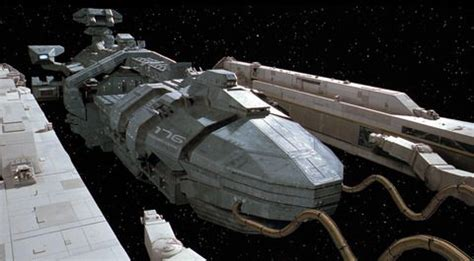
\includegraphics[scale=0.4]{images/spaceShip.jpg}
\end{center}
\\
\end{document}
